% Generated by pysimcount.pfchilds -- do not edit; regenerate instead.
% figure: main-cnot-suzuki-orders -- Suzuki formulas of each order, cnot gates vs n (layout of Childs et al. 2018 Fig. 3 right)
% source: ../np-main/aggregate.json + ../np-main-n9/seed{seed}, ../np-main-n11/seed{seed} (seeds [1, 2, 3, 4, 5, 6, 7, 8, 9, 10]); run commits: 01d3c275ceae2840002bd1aaea68f59b987c4975, e42ff29056ad9ea7fc7c9899fab334903e42e3e3
% metric=cnot kind=xyz merged (cz, simcount template)
% measured n: mean over seeds of the run's totals; bars min..max over seeds
% r from power-law fit to mean measured r (n = 5--11); r = ceil(a n^b); bars = min..max of per-seed fits
% per-step counts exactly affine in n (checked on n = [10, 20, 40], direct build at n = [100])
% shown: suzuki4, suzuki6, suzuki8
% removed (see main-cnot-suzuki-orders-ranking.md): lie-trotter, suzuki2
% figure made at git_commit=e42ff29056ad9ea7fc7c9899fab334903e42e3e3 git_dirty=True
% WARNING: made from uncommitted code; the commit above does not reproduce it.
% derived: main-cnot-suzuki-orders.tex restyled by pysimcount.figuniform: extrapolated points (r from power-law fit) drawn in their series' measured style, style-key legend entries removed; extrapolated n = [13, 20, 30, 50, 70, 100, 200, 300, 500]; source_sha256=7146b51673b9743ed3013c8a4cc4ad8605d044a10f3df14c42aa5c903f213aed
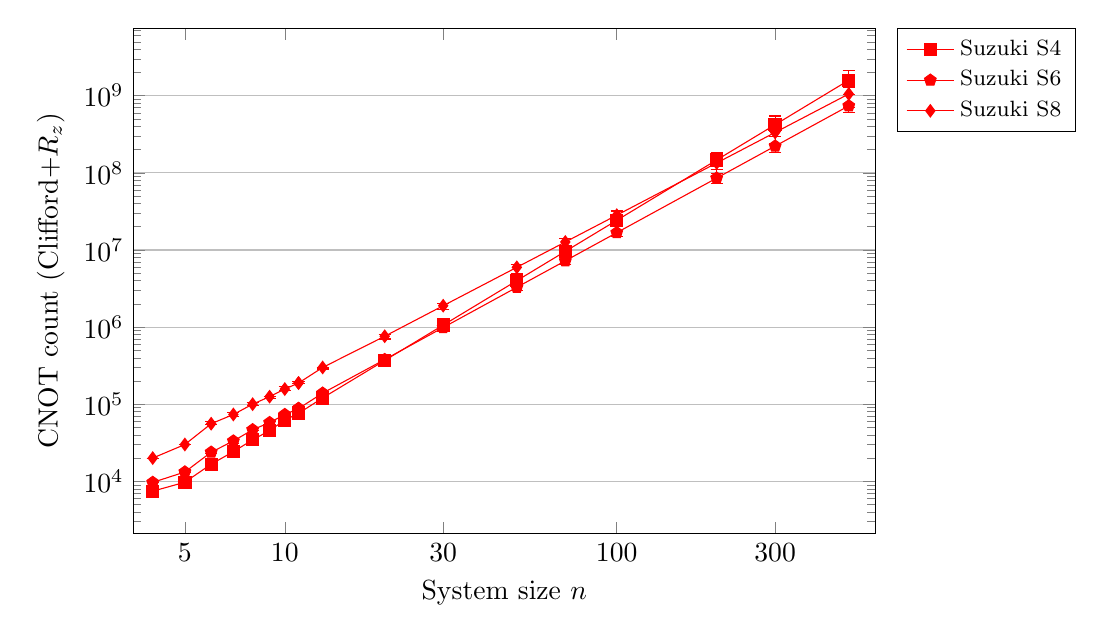
\begin{tikzpicture}
  \begin{loglogaxis}[
    width=11cm, height=8cm,
    xlabel={System size $n$},
    ylabel={CNOT count (Clifford+$R_z$)},
    xtick={5,10,30,100,300}, xticklabels={5,10,30,100,300},
    xmin=3.5, xmax=600,
    ymajorgrids=true,
    legend pos=outer north east,
    legend cell align=left,
    legend style={font=\footnotesize},
  ]
    % suzuki4: measured n, mean over seeds, bars min..max over seeds
    \addplot[red, solid, mark=square*, mark size=2.2pt, mark options={solid, fill=red}, error bars/.cd, y dir=both, y explicit, error bar style={solid}] coordinates {
      (4,7459.2) += (0,100.8) -= (0,67.2)
      (5,9744) += (0,336) -= (0,294)
      (6,16707.6) += (0,1184.4) -= (0,831.6)
      (7,24284.4) += (0,1881.6) -= (0,1646.4)
      (8,34540.8) += (0,1411.2) -= (0,1276.8)
      (9,45549) += (0,2079) -= (0,2457)
      (10,62412) += (0,4788) -= (0,2352)
      (11,76230) += (0,3234) -= (0,1848)
    };
    \addlegendentry{Suzuki S4}
    % suzuki4: extrapolated, r = ceil(3.65267 n^1.59931), per step = 42 n + 0; bars min..max of per-seed fits
    \addplot[red, solid, mark=square*, mark size=2.2pt, mark options={solid, fill=red}, forget plot, error bars/.cd, y dir=both, y explicit, error bar style={solid}] coordinates {
      (11,76230)
      (13,120666) += (0,5460) -= (0,3822)
      (20,369600) += (0,27720) -= (0,20160)
      (30,1.06092e+06) += (0,109620) -= (0,80640)
      (50,4.0005e+06) += (0,575400) -= (0,403200)
      (70,9.59322e+06) += (0,1.63758e+06) -= (0,1.12308e+06)
      (100,2.42382e+07) += (0,4.8552e+06) -= (0,3.2424e+06)
      (200,1.46882e+08) += (0,3.81108e+07) -= (0,2.43096e+07)
      (300,4.21382e+08) += (0,1.24501e+08) -= (0,7.73136e+07)
      (500,1.58972e+09) += (0,5.44026e+08) -= (0,3.26886e+08)
    };
    % suzuki6: measured n, mean over seeds, bars min..max over seeds
    \addplot[red, solid, mark=pentagon*, mark size=2.2pt, mark options={solid, fill=red}, error bars/.cd, y dir=both, y explicit, error bar style={solid}] coordinates {
      (4,9696) += (0,0) -= (0,0)
      (5,13231) += (0,909) -= (0,101)
      (6,23876.4) += (0,1575.6) -= (0,848.4)
      (7,33370.4) += (0,1979.6) -= (0,2262.4)
      (8,46702.4) += (0,1777.6) -= (0,1454.4)
      (9,57812.4) += (0,2181.6) -= (0,3272.4)
      (10,73528) += (0,5252) -= (0,2828)
      (11,87991.2) += (0,3110.8) -= (0,1333.2)
    };
    \addlegendentry{Suzuki S6}
    % suzuki6: extrapolated, r = ceil(1.63295 n^1.35284), per step = 202 n + 0; bars min..max of per-seed fits
    \addplot[red, solid, mark=pentagon*, mark size=2.2pt, mark options={solid, fill=red}, forget plot, error bars/.cd, y dir=both, y explicit, error bar style={solid}] coordinates {
      (11,87991.2)
      (13,139178) += (0,7878) -= (0,2626)
      (20,379760) += (0,32320) -= (0,12120)
      (30,987780) += (0,115140) -= (0,54540)
      (50,3.2825e+06) += (0,535300) -= (0,272700)
      (70,7.23968e+06) += (0,1.39986e+06) -= (0,721140)
      (100,1.6766e+07) += (0,3.7774e+06) -= (0,1.9594e+06)
      (200,8.55672e+07) += (0,2.50884e+07) -= (0,1.2726e+07)
      (300,2.2216e+08) += (0,7.41138e+07) -= (0,3.71478e+07)
      (500,7.38916e+08) += (0,2.8583e+08) -= (0,1.40087e+08)
    };
    % suzuki8: measured n, mean over seeds, bars min..max over seeds
    \addplot[red, solid, mark=diamond*, mark size=2.2pt, mark options={solid, fill=red}, error bars/.cd, y dir=both, y explicit, error bar style={solid}] coordinates {
      (4,20040) += (0,0) -= (0,0)
      (5,30060) += (0,0) -= (0,0)
      (6,55911.6) += (0,4208.4) -= (0,1803.6)
      (7,73647) += (0,3507) -= (0,3507)
      (8,100200) += (0,4008) -= (0,4008)
      (9,125350) += (0,901.8) -= (0,8116.2)
      (10,157314) += (0,13026) -= (0,7014)
      (11,188476) += (0,9919.8) -= (0,1102.2)
    };
    \addlegendentry{Suzuki S8}
    % suzuki8: extrapolated, r = ceil(0.896539 n^1.24879), per step = 1002 n + 0; bars min..max of per-seed fits
    \addplot[red, solid, mark=diamond*, mark size=2.2pt, mark options={solid, fill=red}, forget plot, error bars/.cd, y dir=both, y explicit, error bar style={solid}] coordinates {
      (11,188476)
      (13,299598) += (0,0) -= (0,13026)
      (20,761520) += (0,40080) -= (0,60120)
      (30,1.89378e+06) += (0,150300) -= (0,210420)
      (50,5.9619e+06) += (0,601200) -= (0,951900)
      (70,1.26953e+07) += (0,1.47294e+06) -= (0,2.31462e+06)
      (100,2.82564e+07) += (0,3.8076e+06) -= (0,5.9118e+06)
      (200,1.34268e+08) += (0,2.26452e+07) -= (0,3.507e+07)
      (300,3.34267e+08) += (0,6.34266e+07) -= (0,9.70938e+07)
      (500,1.0541e+09) += (0,2.29458e+08) -= (0,3.41682e+08)
    };
  \end{loglogaxis}
\end{tikzpicture}
